\documentclass[a4paper,11pt,fleqn]{article}%fleqn pour aligner les equations à gauche
\usepackage{../../Styles/Cours}

\newcommand{\chnum}{Chapitre 17}
\newcommand{\chtitle}{Propagation des ondes}
\newcommand{\dtype}{Cours}


\begin{document}
\maketitle

\section{Atténuation des ondes sonores}
	\subsection{Intensité sonore}
	\begin{minipage}{.7\textwidth}
	Une onde sonore, comme toute onde, transporte de l'énergie (donc de la puissance). Cette énergie et cette puissance se répartissent sur une surface sphérique autour de la source. On définit l'intensité sonore $I$ comme la puissance sonore $P$ émise par une source sur une surface $S$ donnée :
	$$I = \dfrac{P}{S} = \dfrac{P}{4\pi d^2} \nonumber$$
	\end{minipage}
	\begin{minipage}{.2\textwidth}
	\begin{tikzpicture}
\fill [blue!40] (0,0) ellipse(2 and .75);

\fill [blue!40] (0,0) circle (2);
\draw [white] (0,0) ellipse(2 and .75);
\draw (0,0) node[white]{$\bullet$} node[below left,  white]{$P$};
\draw (0,0) node[above left,  white]{Source};
\draw [<->,white] (0,0) to (1.9,0.7);
\draw [white](0.95,.1) node{$d$};

\draw (2.7,.8) node{$I=\dfrac{P}{S}$};
\draw (1,2.3) node{$S=4\pi d^2$};
\end{tikzpicture}
	\end{minipage}
	
	\subsection{Niveau d'intensité sonore}
	\begin{minipage}{.4\linewidth}
	Une intensité deux fois plus importante ne donne pas une sensation d'un son deux fois plus fort. La perception du volume sonore n'est pas proportionnelle à l'intensité. Pour modéliser ce fait physiologique, on définit le niveau d'intensité sonore $L$ à l'aide d'une échelle logarithmique :
	$$L = 10\cdot \log \left(\dfrac{I}{I_0}\right)$$
	Le niveau d'intensité sonore est défini par rapport à l'intensité sonore de référence $I_0$, intensité la plus faible qu'une oreille normale puisse entendre. $I_0$ = \SI{1,0E-12}{\watt \per \meter \squared}
	\end{minipage}
	\begin{minipage}{.5\linewidth}
		\begin{tikzpicture}
		\draw (-3,11) node{\textbf{Niveau sonore $\mathbf{L}$(dB)}};
		\draw (1.5,11) node{\textbf{Intensité sonore $\mathbf{I}$(\unit{\watt\per\meter\squared})}};

		\fill[green!30!gray] (0,-.5) rectangle(.5,5);
		\fill[orange!90!gray] (0,5) rectangle(.5,6);
		\fill[red!70!gray] (0,6) rectangle(.5,8.5);
		\fill[brown!50!black] (0,8.5) rectangle(.5,10.5);
		\draw (0,-0.5) rectangle(.5,10.5);
		
		\foreach \k/\v/\l/\a in {
			0/\num{1E-9}/\num{30}/,
			1/\num{1E-8}/\num{40}/Bibliothèque,
			2/\num{1E-7}/\num{50}/,
			3/\num{1E-6}/\num{60}/Lave-linge,
			4/\num{1E-5}/\num{70}/Aspirateur,
			5/\num{1E-4}/\num{80}/Cours de récréation,
			6/\num{1E-3}/\num{90}/Perceuse,
			7/\num{1E-2}/\num{100}/Tronçonneuse,
			8/\num{1E-1}/\num{110}/Marteau-piqueur,
			8.5/\num{3E-1}/\num{115}/Seuil de douleur,
			9/\num{1}/\num{120}/Coup de fusil,
			10/\num{10}/\num{130}/Avion au décollage}{
			\draw (-.2,\k) -- (.7,\k);
			\draw (-1,\k) node{\v};
			\draw (-3,\k) node{\l};
			\draw (3,\k) node{\a};
		}

		\filldraw[black, green!30!gray] (-3,-1) rectangle(-2.25,-0.75);
		\filldraw[black, orange!90!gray] (-3,-2) rectangle(-2.25,-1.75);
		
		\filldraw[black, red!70!gray] (1,-1) rectangle(1.75,-0.75);
		\filldraw[black, brown!50!black] (1,-2) rectangle(1.75,-1.75);

		\draw (-1,-.9) node{Pas de risque};
		\draw (-.7,-1.9) node{Limite de nocivité};

		\draw (3.65,-.9) node{Danger : sons nocifs};
		\draw (3.9,-1.9) node{Dommages irréversibles};
		
		\end{tikzpicture}	
	\end{minipage}

\newpage
	\subsection{Atténuation}
	Le niveau d'intensité sonore diminue :
	\begin{itemize}
		\item Lorsque l'on s'éloigne de la source car la surface sur laquelle est répartie la puissance sonore est plus grande. On parle alors d'\textbf{atténuation géométrique}.
		\item Lorsque l'onde sonore se propage dans un milieu absorbant, une partie de l'énergie est alors transférée au matériau. On parle d'\textbf{atténuation par absorption}.
	\end{itemize}
    Pour qualifier ce phénomène, on définit $A$ l'atténuation :
    $$A=L_{sortie}-L_{entrée} = 10\cdot Log\left(\dfrac{I_{sortie}}{I_{entree}}\right)$$
\section{Effet Doppler}
\subsection{Manifestation}
Lorsque la source d'une onde périodique (sonore ou lumineuse) est en mouvement par rapport à l'observateur, la fréquence du signal reçu par l'observateur est différente de celle du signal émis apr la source.\\
Lorsque la source se déplace, la distance entre les crêtes de l'onde se réduit dans le sens du déplacement (la source s'est rapprochée de la crête émise précédemment durant le temps écoulé entre l'émission des deux crêtes) et augmente dans le sens inverse (la source s'est éloignée de la crête précédemment durant le temps écoulé entre l'émission des deux crêtes).

\noindent\colorbox{blue!10}{
	\begin{minipage}{.98\linewidth}
        Ainsi, si la source se rapproche, la fréquence reçue est plus élevée que celle émise (le son est donc aigu) et inversement si la source s'éloigne. Ce décalage en fréquence est appelé effet Doppler. Il est d'autant plus important que la vitesse est grande.
    \end{minipage}
}
Dans la limite où la source atteint la vitesse de propagation de l'onde ($v=v_{onde}$), l'onde n'est plus périodique ($f=\SI{0}{\hertz}$), car la source "rattrape" l'onde. Ce cas peut se présenter, par exemple, pour les avions de chasse lorsqu'ils franchissent le mur du son.

\begin{figure}[h!]
	\centering
	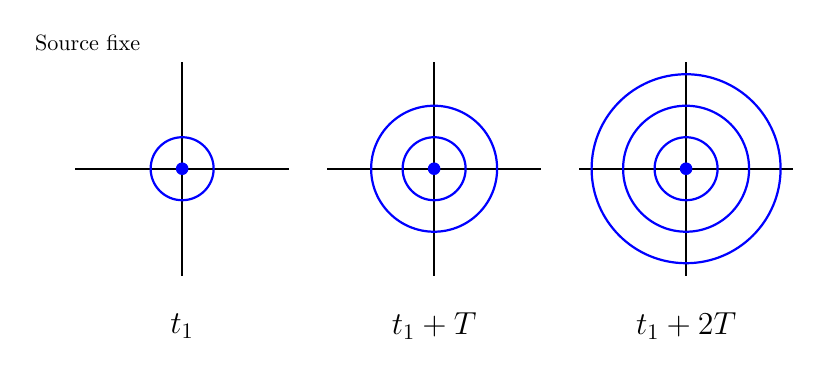
\begin{tikzpicture}[scale=.8,transform shape]
		\draw (0,2) node{Source fixe};

		\draw[thick] (-.2,0) -- (3.2,0);
		\draw[thick] (1.5,-1.7) -- (1.5,1.7);
		\fill[blue] (1.5,0) circle(.1);
		\draw[blue, thick] (1.5,0) circle(.5);

		\draw[thick] (3.8,0) -- (7.2,0);
		\draw[thick] (5.5,-1.7) -- (5.5,1.7);
		\fill[blue] (5.5,0) circle(.1);
		\draw[blue, thick] (5.5,0) circle(.5);
		\draw[blue, thick] (5.5,0) circle(1);

		\draw[thick] (7.8,0) -- (11.2,0);
		\draw[thick] (9.5,-1.7) -- (9.5,1.7);
		\fill[blue] (9.5,0) circle(.1);
		\draw[blue, thick] (9.5,0) circle(.5);
		\draw[blue, thick] (9.5,0) circle(1);
		\draw[blue, thick] (9.5,0) circle(1.5);

		\draw (1.5,-2.5) node{\Large$t_1$};
		\draw (5.5,-2.5) node{\Large$t_1+T$};
		\draw (9.5,-2.5) node{\Large$t_1+2T$};
	\end{tikzpicture}
	
	\vspace{1em}
	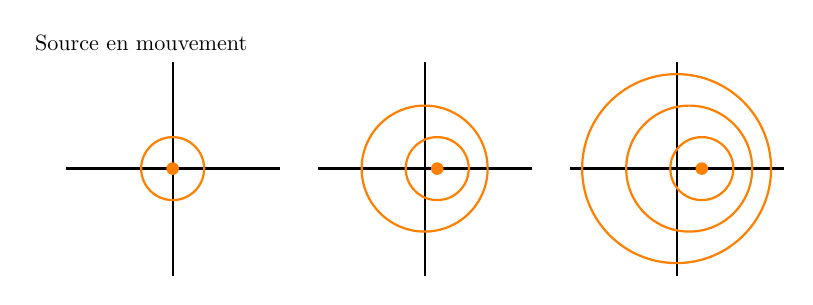
\begin{tikzpicture}[scale=.8,transform shape]
		\draw (1,2) node{Source en mouvement};

		\draw[thick] (-.2,0) -- (3.2,0);
		\draw[thick] (1.5,-1.7) -- (1.5,1.7);
		\fill[orange] (1.5,0) circle(.1);
		\draw[orange, thick] (1.5,0) circle(.5);

		\draw[thick] (3.8,0) -- (7.2,0);
		\draw[thick] (5.5,-1.7) -- (5.5,1.7);
		\fill[orange] (5.7,0) circle(.1);
		\draw[orange, thick] (5.7,0) circle(.5);
		\draw[orange, thick] (5.5,0) circle(1);

		\draw[thick] (7.8,0) -- (11.2,0);
		\draw[thick] (9.5,-1.7) -- (9.5,1.7);
		\fill[orange] (9.9,0) circle(.1);
		\draw[orange, thick] (9.9,0) circle(.5);
		\draw[orange, thick] (9.7,0) circle(1);
		\draw[orange, thick] (9.5,0) circle(1.5);
	\end{tikzpicture}
\end{figure}

\subsection{Fréquence reçue par le récepteur}
Un observateur fixe observe une source se déplaçant à une vitesse $v$ dans sa direction et émettant des bips avec une période $T_{em}$.\\
Entre l'émission d'un bip et le suivant, le premier bip s'est déplacé d'une distance $d_1=v_{onde}\cdot T_{em}$, mais la source s'est déplacée d'une distance $d_2=v\cdot T_{em}$. Par conséquent, la longueur d'onde, qui est la distance sépatant les deux bips, est :
\begin{itemize}
	\item si la source se rapproche de l'observateur : $$\lambda = d_1 - d_2 = (v_{onde} - v) \cdot T_{em} = \dfrac{v_{onde}-v}{f_{em}}$$
	\item si la source s'éloigne de l'observateur : $$\lambda = d_1 - d_2 = (v_{onde} + v) \cdot T_{em} = \dfrac{v_{onde}+v}{f_{em}}$$
\end{itemize}

Par conséquent, la fréquence reçue par l'observateur est égale à :
\begin{itemize}
	\item si la source se rapproche : $$f_{rec}=f_{em}\cdot \dfrac{v_{onde}}{v_{onde}-v} = \dfrac{f_{em}}{1-\dfrac{v}{v_{onde}}}$$
	\item si la source d'éloigne : $$f_{rec}=f_{em}\cdot \dfrac{v_{onde}}{v_{onde}+v} = \dfrac{f_{em}}{1+\dfrac{v}{v_{onde}}}$$
\end{itemize}

\subsection{Décalage Doppler en fréquence}
Le \textbf{décalage Doppler} est la différence $\Delta f$ entre la fréquence $f_{rec}$ perçue par l'observateur et la fréquence $f_{em}$ émise par la source.
\begin{itemize}
	\item $\Delta f = f_{rec} - f_{em}> \SI{0}{\hertz}$ si la source s'approche.
	\item $\Delta f = f_{rec} - f_{em}< \SI{0}{\hertz}$ si la source s'éloigne.
\end{itemize}

Dans le cas où la vitesse de la source est très faible devant celle de l'onde ($v<<v_{onde}$), on peut écrire l'approximation :
$$ |\Delta f | = \dfrac{v}{v_{onde}} \cdot f_{em}$$
Dans le cas où le récepteur est fixe par rapport à l'émetteur er reçoit une onde réfléchie par un objet en mouvement, le décalage Doppler a lieu deux fois (entre l'émetteur et l'objet, puis entre l'objet et le récepteur) et un facteur 2 apparaît dans la formule.

\subsection{Décalage Doppler en longueur d'onde}

Pour les ondes électromagnétiques, la célérité de l'onde est la même pour l'émetteur et le récepteur, mais la fréquence et la longueur d'onde sont différentes. Ainsi, on observe des décalages en longueur d'onde des raies caractéristiques des spectres d'absorption des étoiles : on parle d'effet \textbf{Doppler-Fizeau}.
\end{document}